%%%%%%%%%%%%%%%%%%%%%%%%%%%%%%%%%%%%%%%%%%%%%%%%%%%%%%%%%%%%%
%% HEADER
%%%%%%%%%%%%%%%%%%%%%%%%%%%%%%%%%%%%%%%%%%%%%%%%%%%%%%%%%%%%%
\documentclass[a4paper,twoside,11pt]{article}

%% Language %%%%%%%%%%%%%%%%%%%%%%%%%%%%%%%%%%%%%%%%%%%%%%%%%
\usepackage[T1]{fontenc}

%\usepackage[ansinew]{inputenc}
\usepackage[utf8]{inputenc}	%supports Umlaute
\usepackage{german, ngerman}
\usepackage{color}

\usepackage{lmodern} %Type1-font for non-english texts and characters

%% Packages for Graphics & Figures %%%%%%%%%%%%%%%%%%%%%%%%%%
\usepackage{graphicx} %%For loading graphic files
\usepackage{multicol}

%% Math Packages %%%%%%%%%%%%%%%%%%%%%%%%%%%%%%%%%%%%%%%%%%%%
\usepackage{amsmath}
\usepackage{amsthm}
\usepackage{amsfonts}
\usepackage{amssymb}

%% Line Spacing %%%%%%%%%%%%%%%%%%%%%%%%%%%%%%%%%%%%%%%%%%%%%
\usepackage[parfill]{parskip}    % Activate to begin paragraphs with an empty line rather than an indent

%% Other Packages %%%%%%%%%%%%%%%%%%%%%%%%%%%%%%%%%%%%%%%%%%%
\usepackage{a4wide} %%Smaller margins = more text per page.
\usepackage{fancyhdr} %%Fancy headings

%%%%%%%%%%%%%%%%%%%%%%%%%%%%%%%%%%%%%%%%%%%%%%%%%%%%%%%%%%%%%
%% DOCUMENT
%%%%%%%%%%%%%%%%%%%%%%%%%%%%%%%%%%%%%%%%%%%%%%%%%%%%%%%%%%%%%
\begin{document}

\pagestyle{fancyplain}

%% Title Page %%%%%%%%%%%%%%%%%%%%%%%%%%%%%%%%%%%%%%%%%%%%%%%
\title{Parallel Programming Assignment \#1} 
\author{Marcel Karsten -- 343619,\\ Patrick Lorenz -- 341922,\\ Richard Klemm -- 343635 }
\date{Due: Thursday, 03th January 2012} %%If commented, the current date is used.
\maketitle

%% Header on top of every page (yes, also on the title page!)
\rhead{Parallel Programming - TU Berlin, SS/12}
\lhead{}
\renewcommand{\headrulewidth}{0px}


%%%%%%%%%%%%%%%%%%%%%%%%%%%%%%%%%%%%%%%%%%%%%%%%%%%%%%%%%%%%%

\section{Exercise 3}
\textbf{(a)}
\begin{figure}[!htbp]
    \begin{center}
        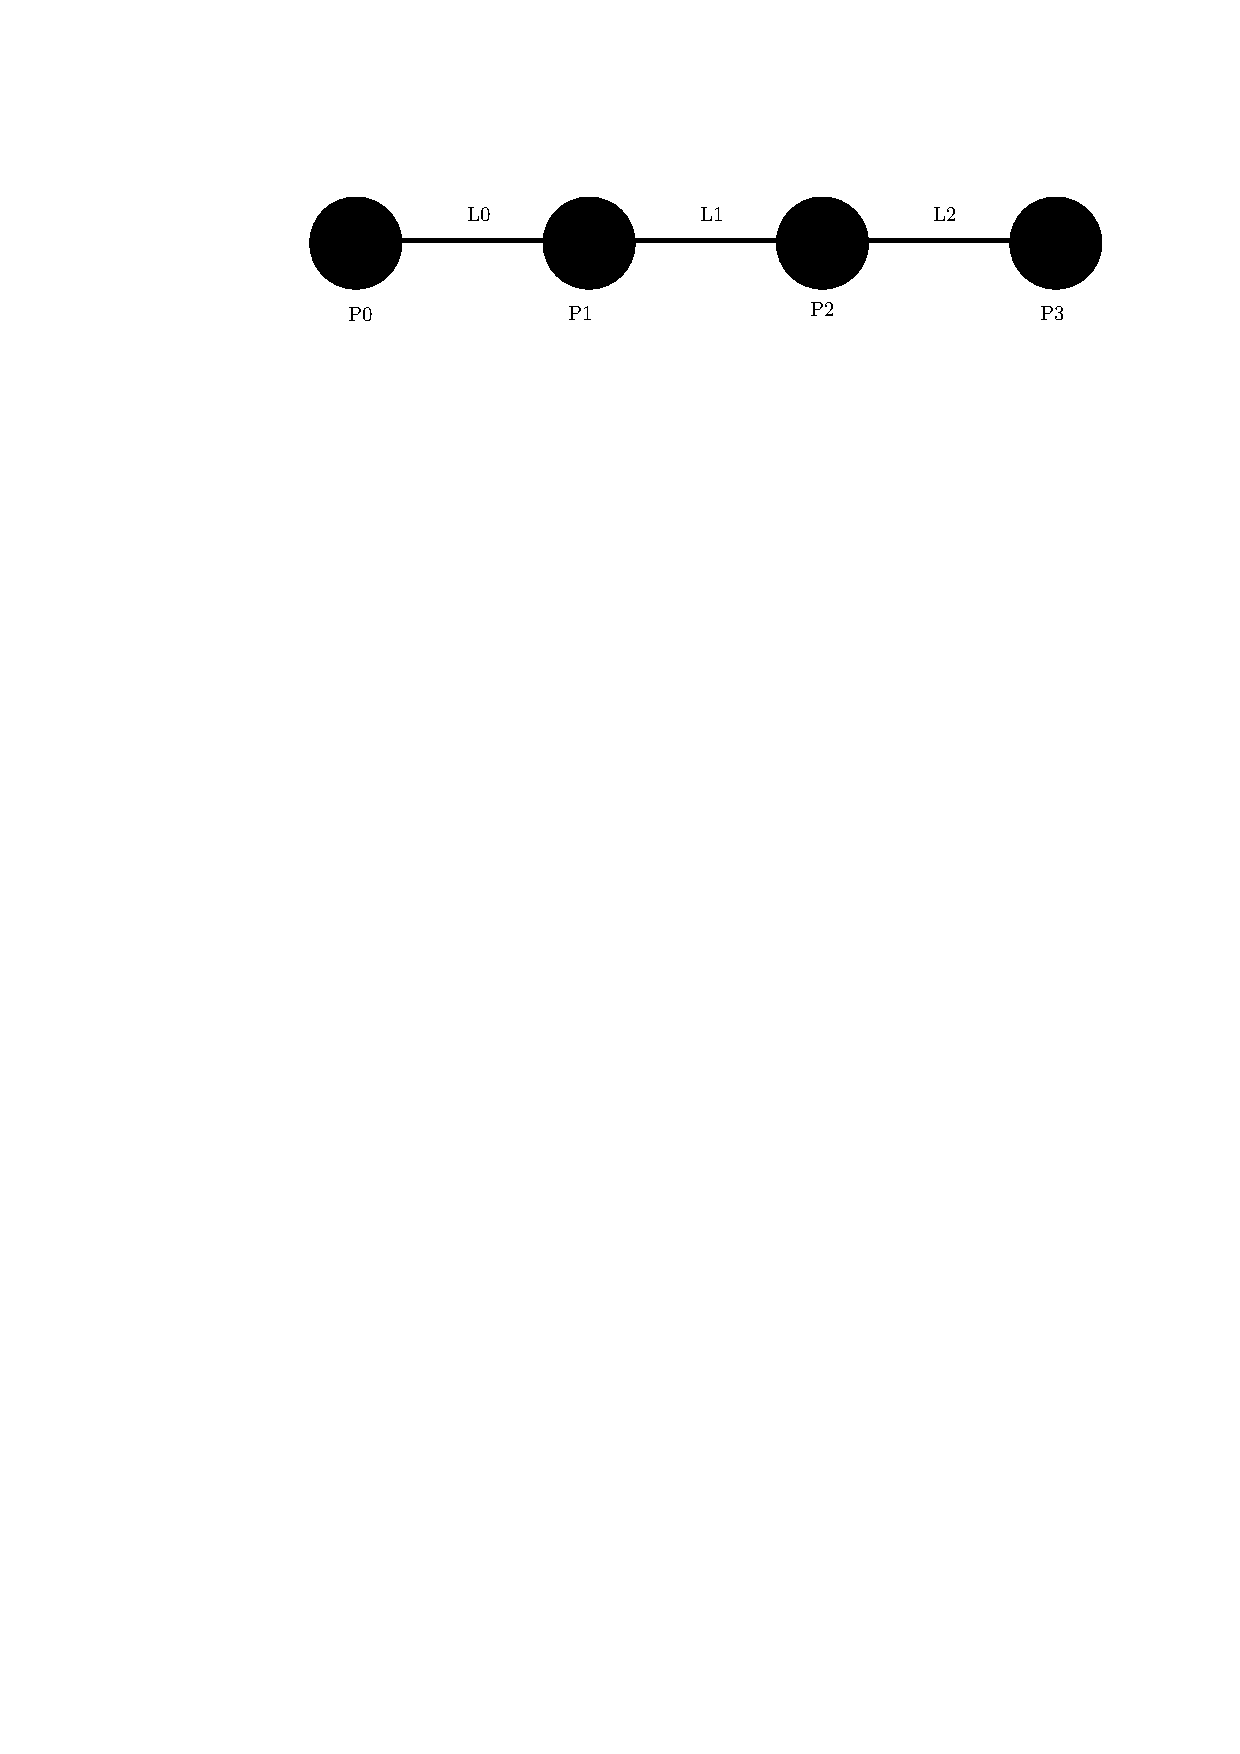
\includegraphics[scale=1]{3a_1.pdf}
    \end{center}
    \caption{Sample Setup}
    \label{SampleSetup}
\end{figure}

It can easily be seen in [Figure \ref{SampleSetup}], it takes $\sum\limits_{i=0}^m L_i$ where $L$ is the delay between two nodes.
With the parameters given, $L_i$ can be described as $\alpha_i + \frac{n_i}{\beta_i}$ where $i$ is in range $0 .. p-1$.
Therefore, the final equation is: $\sum\limits_{i=0}^{p-1} \alpha_i + \frac{n_i}{\beta_i}$.
As L is unchanged this is equal to: $M = (p-1) * (\alpha + \frac{n}{\beta})$, with M being the message delay.
\\\\
\textbf{(c)\\ 1.}\hspace{1em}\\Another idea to broadcast the messages is to use a binary tree.
\begin{figure}[!htbp]
    \begin{center}
        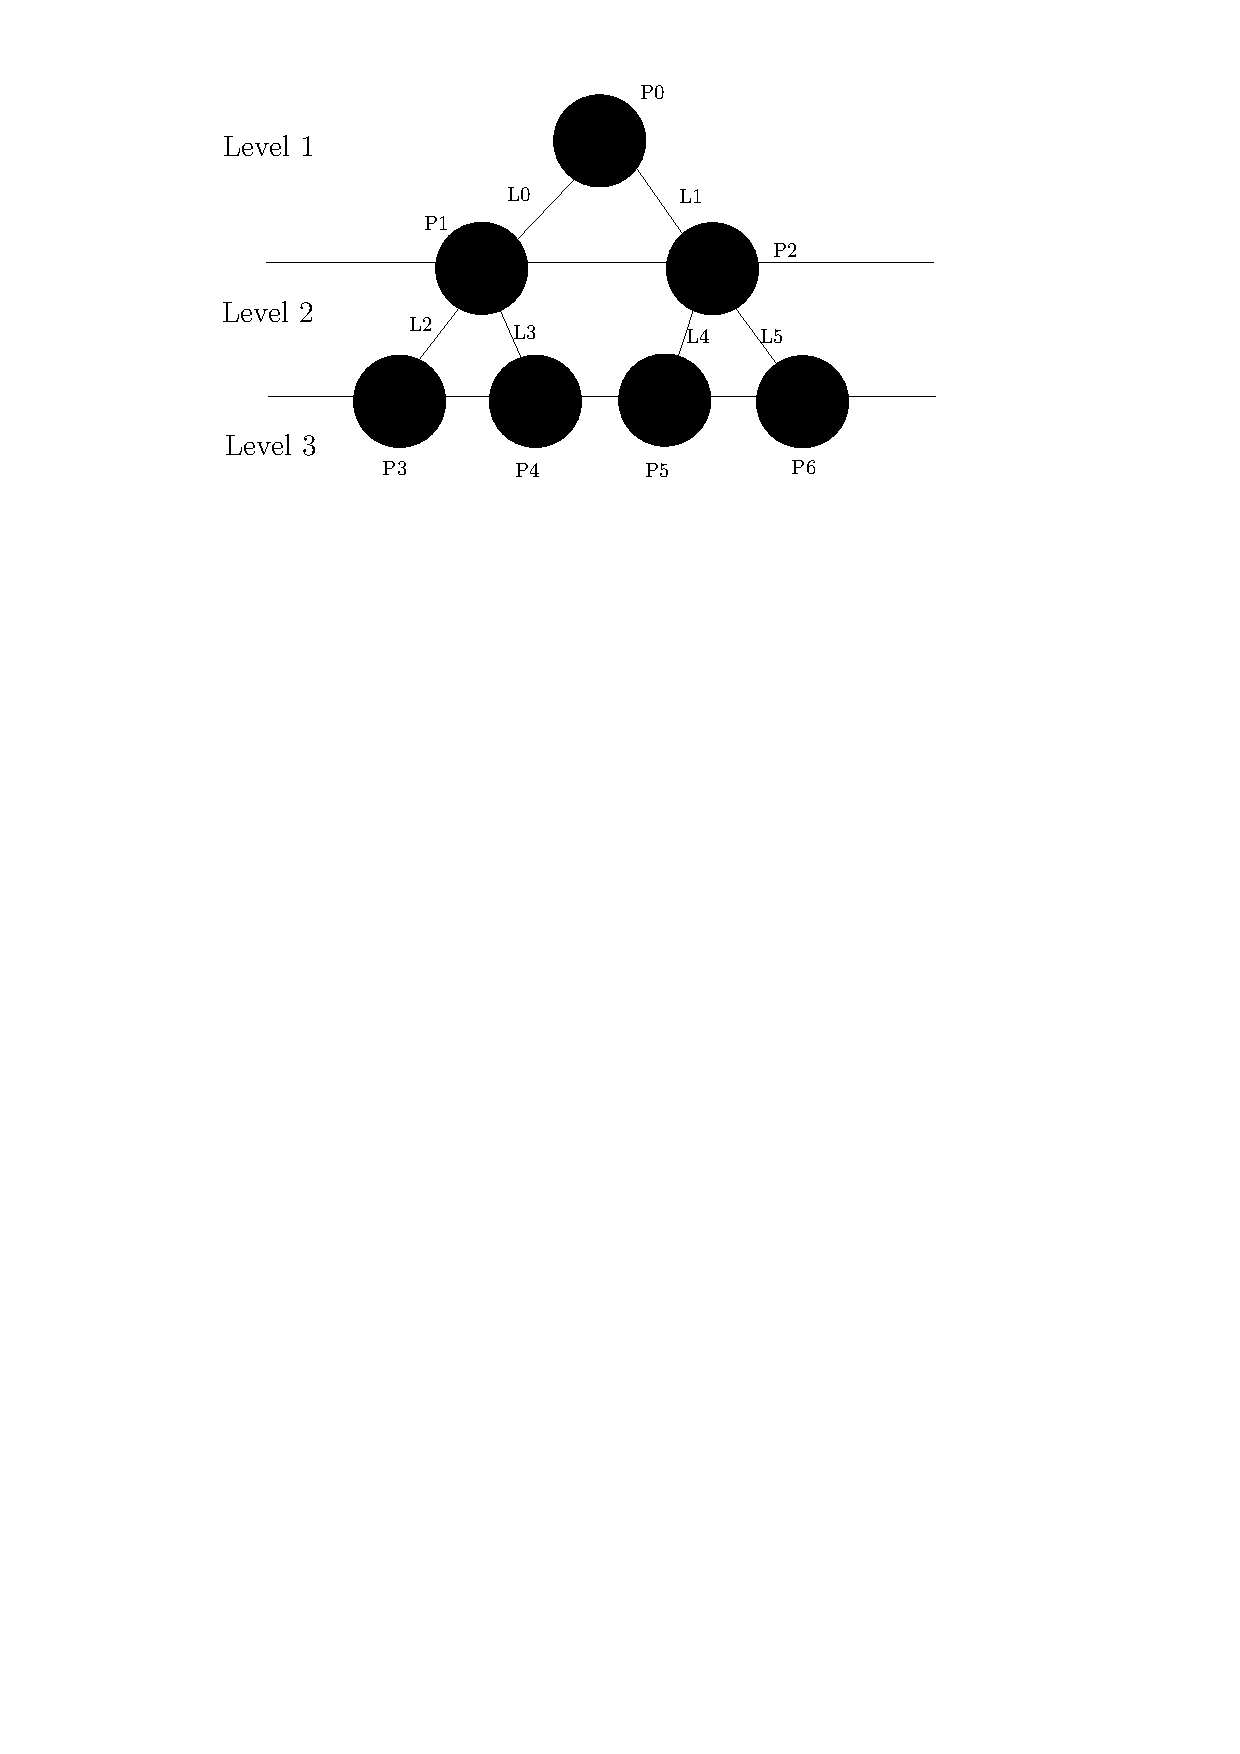
\includegraphics[scale=1]{3c_1.pdf}
    \end{center}
    \caption{Sample Binary Tree}
    \label{BinTree}
\end{figure}
The binary tree has a number of nice properties, that are interesting for message passing.
One of which is $p-1=2^h$, where  $h$ is the depth of the tree and $p$ the number of processes.

Nodes belonging to the same level can work in parallel, thus the problem can be reduced to a tree as seen in [Figure: \ref{SubBinTree}]
It can easily be seen, that a node can at most send two messages. Thus $M = 2Lh$.
$h$ can be acquired by re-arranging the equation given above: $h=\log_2 (p-1)$
Thus, the final equation for estimating $M$ is $M= 2*(\alpha_i + \frac{n_i}{\beta_i}) * \log_2 (p-1)$


\begin{figure}[!htbp]
    \begin{center}
        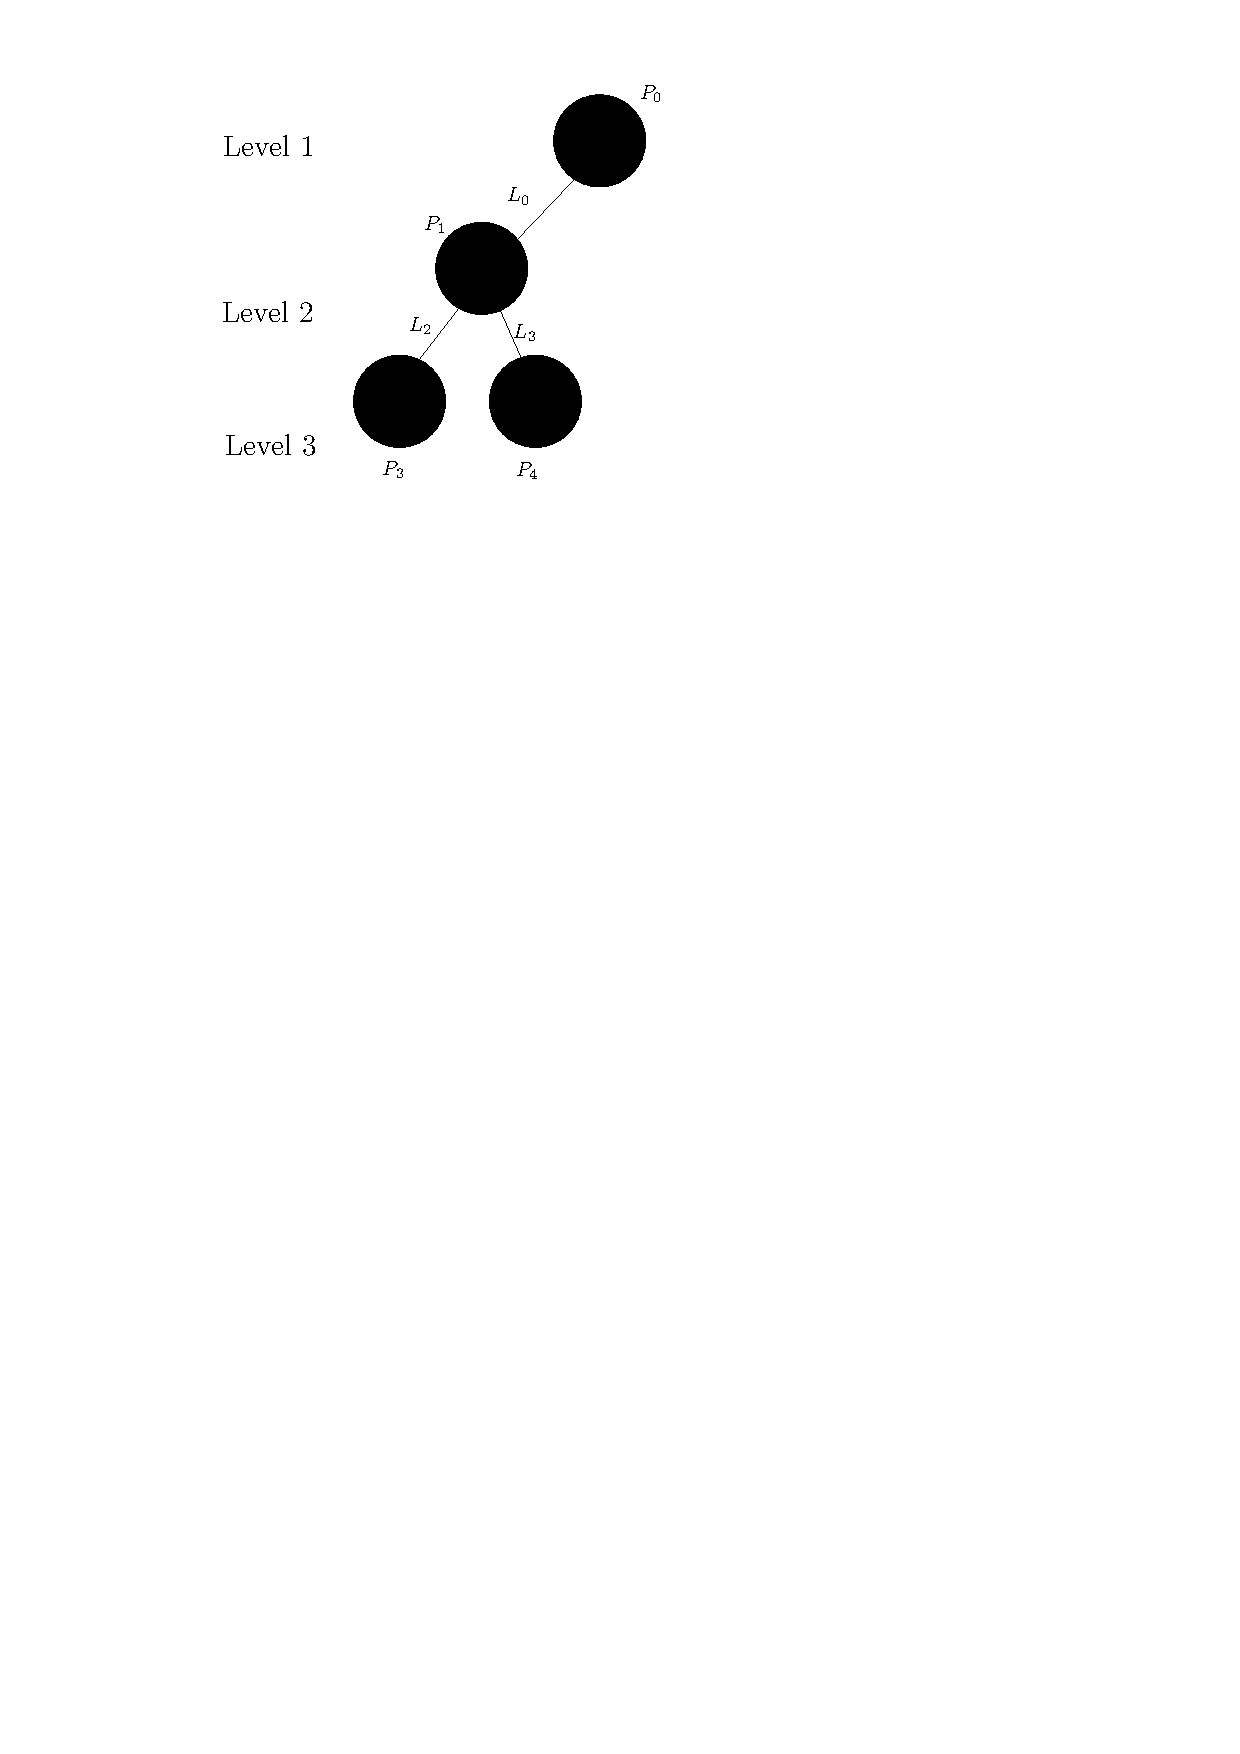
\includegraphics[scale=1]{3c_2.pdf}
    \end{center}
    \caption{Sub Binary Tree}
    \label{SubBinTree}
\end{figure}

\textbf{2.}

Yet another alternative is using a simple star structure.
$P_0$ sends a message to all the other nodes.
As broadcast is not allowed the message delay can be calculated in short: \mbox{$M = (p-1)*L$} or with $L$ substituted: $M = (p-1) * (\alpha_i + \frac{n_i}{\beta_i})$
\begin{figure}[!htbp]
    \begin{center}
        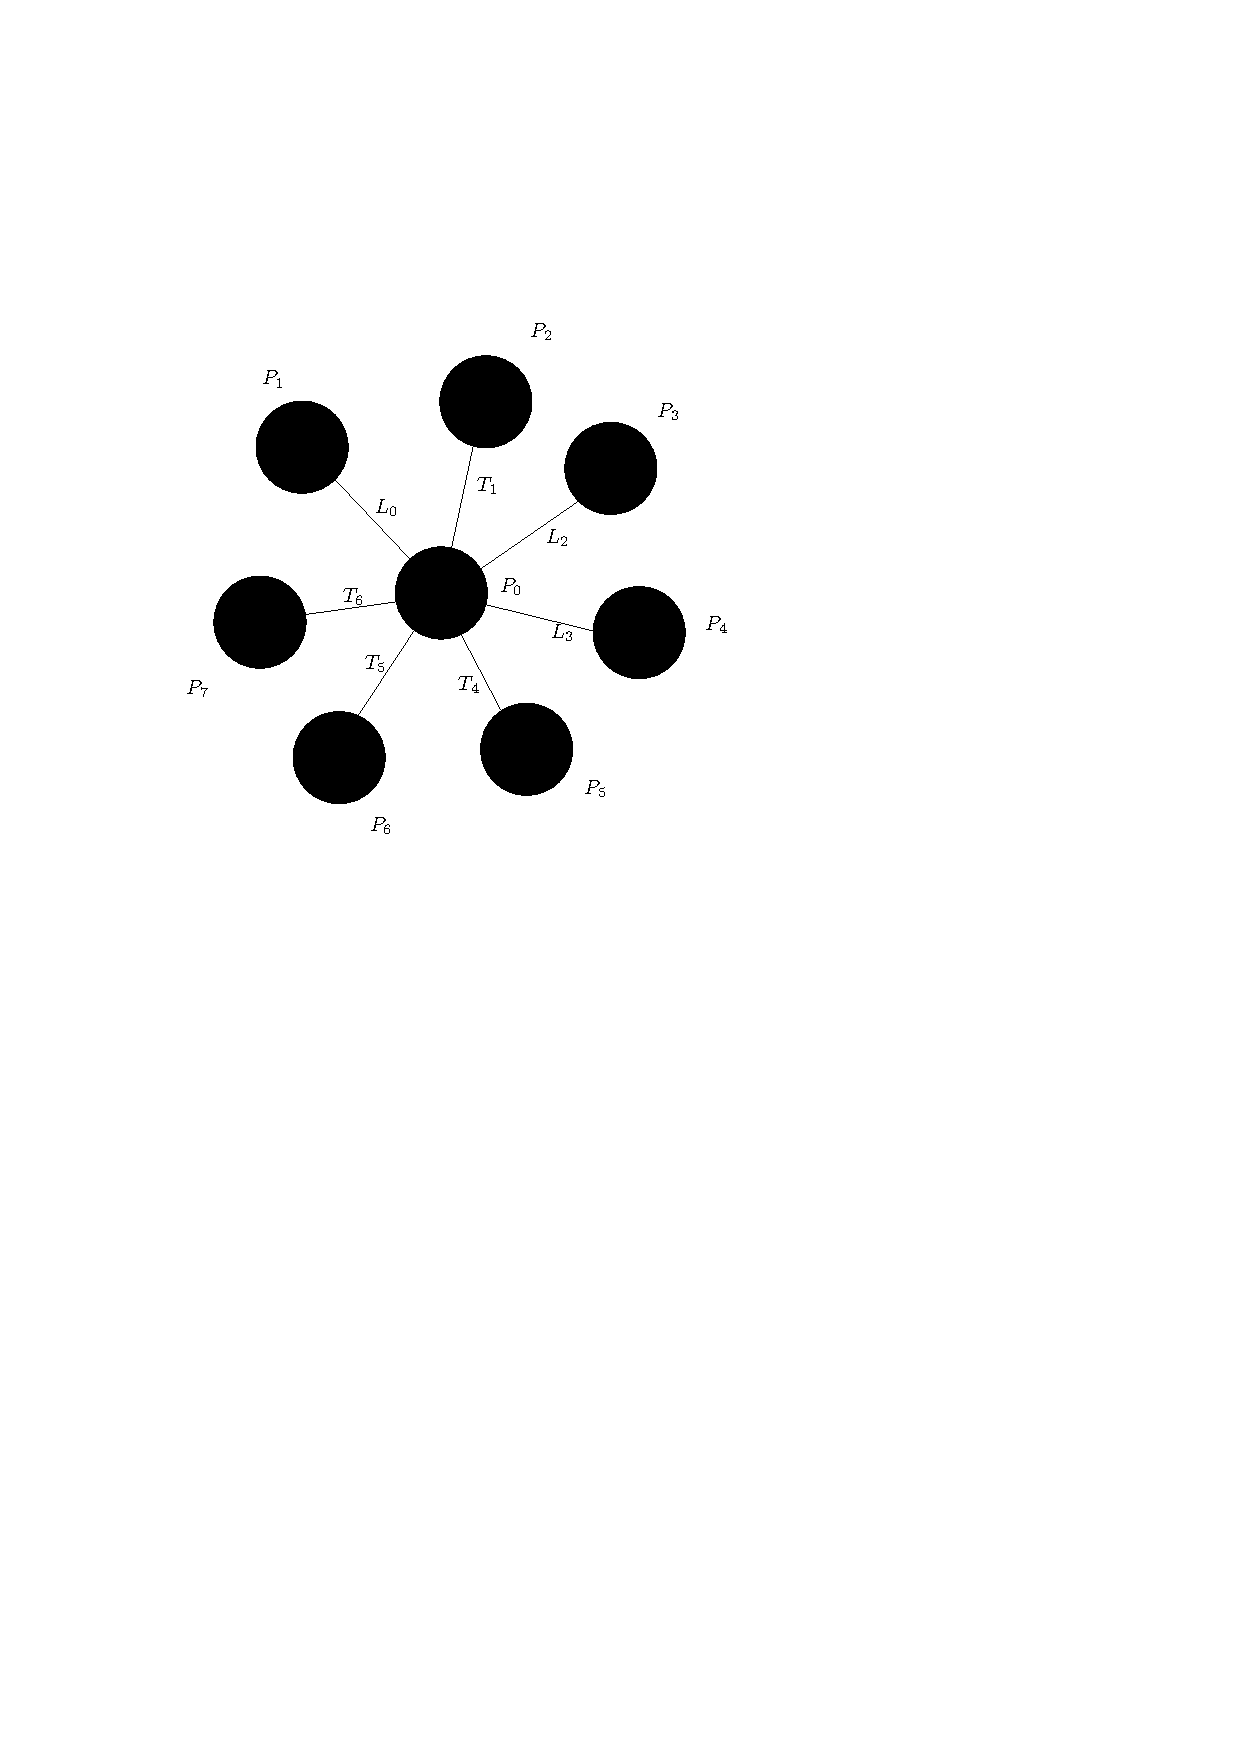
\includegraphics[scale=1]{3c_3.pdf}
    \end{center}
    \caption{Star}
    \label{Star}
\end{figure}



$ $ \\
\textbf{How latency, bandwidth and message size influence performance}

\hspace{1em}Latency is a constant factor, that just adds to the overall delay. (See equation above). Message size and bandwidth correlate to each other in a way that they can be left out of the equation if the bandwidth is just big enough.
The formula $\frac{messagesize}{bandwith}$ converges to 0 if the bandwidth is just big enough. Also, if there is not enough bandwidth available, the message size should be kept as small as possible to get a good performance.


\end{document}
